\begin{frame}
  \frametitle{Resources}
  %\framesubtitle{If you want to improve this style}
  \begin{thebibliography}{10}

  \beamertemplatearticlebibitems

  \bibitem{PEPS}
  A Practical Introduction to Tensor Networks
    \newblock {\tt Orus, R. A Practical Introduction to Tensor Networks: Matrix Product States and Projected Entangled Pair States. arXiv [cond-mat.str-el] (2013). at <http://arxiv.org/abs/1306.2164> 
}

  \end{thebibliography}
\end{frame}

\frame{
  \vspace{2cm}
  {\huge Questions ?}

  \vspace{3cm}
  \begin{flushright}
    Brayden Ware

    \structure{\footnotesize{brayden@physics.ucsb.edu}}
  \end{flushright}
}

\frame{
  \vfill
  \centering
  \highlighton{
  \usebeamerfont*{frametitle}Bonus slides

  \usebeamerfont*{framesubtitle}Bonus slides
  }
  \vfill
}

\begin{frame}{RVB States}
\begin{figure}
\centering
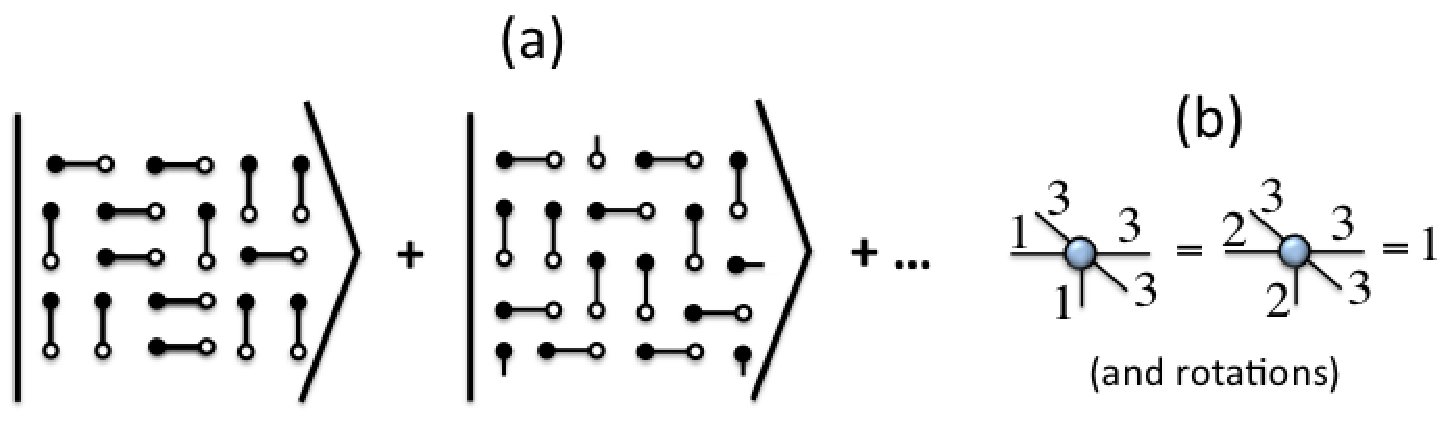
\includegraphics[width=\textwidth]{orus-images/fig30.pdf}
\end{figure}
\end{frame}